\section{Généralités sur l'administration sous Linux}
%Sacha

\subsection{GNU/Linux}

\begin{frame}{GNU/Linux}

\begin{itemize}
\item Linux est un noyau de syst�me d'exploitation
\begin{itemize} \item Initi� par Linux Torvald \end{itemize}
\item GNU est un syst�me d'exploitation
i\item \begin{itemize} \item Initi� par Richard Stallman \end{itemize}
\item GNU/Linux = GNU over Linux
\end{itemize}

\end{frame}

\frame{\frametitle{GNU/Linux}
		\framesubtitle{Architecture GNU/Linux}
  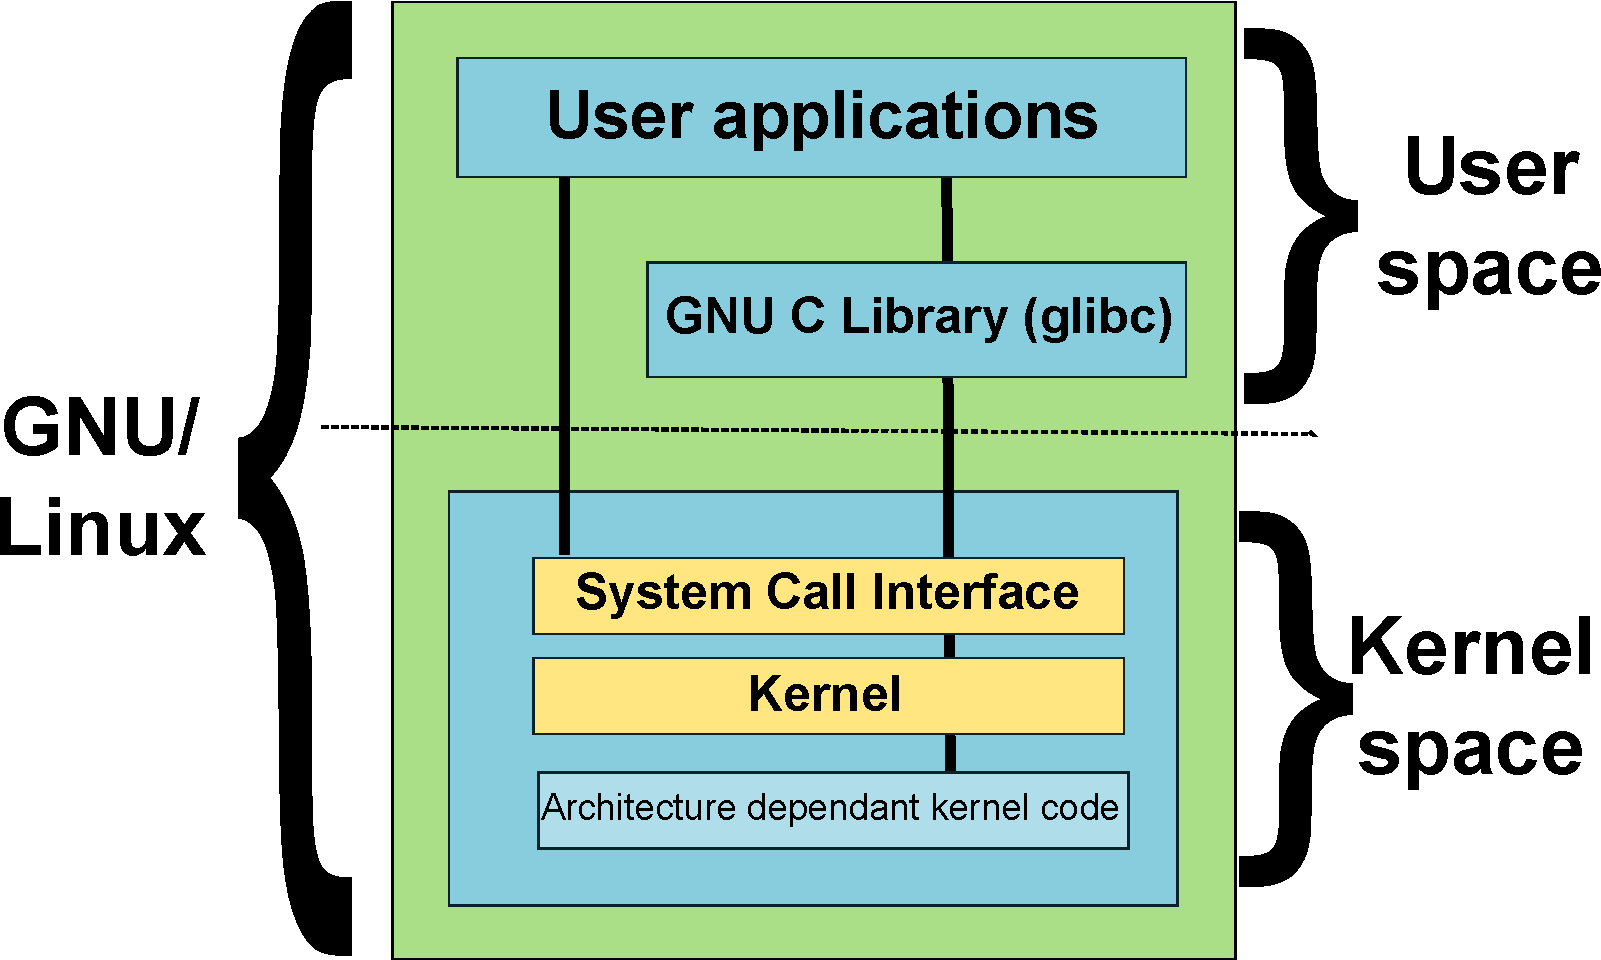
\includegraphics[scale=0.25]{Images/gnulinux.pdf}
}


\subsection{Distribution linux}
\begin{frame}{Distribution linux}

\begin{itemize}
\item Distribution GNU/Linux = Noyaux Linux + Utilitaire et biblioth�ques GNU + ...
\begin{itemize} \item Un syst�me d'exploitation compos� d'un ensemble de logiciels stable et coh�rent  \end{itemize}
\item Trois familles historiques de distributions linux :
  \begin{itemize}
    \item Debian (Debian, Ubuntu, Knopix, etc.)
    \item Slackware (Slackware, S.u.S.E, openSuse, etc.)
    \item Red Hat (Red Hat Enterprise, Mandriva, Fedora, etc...)
  \end{itemize}
\end{itemize}

\end{frame}

\subsection{Debian GNU/Linux}
\begin{frame}{Debian GNU/Linux}

\begin{itemize}
\item 
\begin{itemize} \item Un syst�me d'exploitation compos� d'un ensemble de logiciels stable et coh�rent  \end{itemize}
\item Trois familles historiques de distributions linux :
  \begin{itemize}
    \item Debian (Debian, Ubuntu, Knopix, etc.)
    \item Slackware (Slackware, S.u.S.E, openSuse, etc.)
    \item Red Hat (Red Hat Enterprise, Mandriva, Fedora, etc...)
  \end{itemize}
\end{itemize}

\end{frame}


\begin{frame}{Commandes de base sous linux}

\begin{itemize}
  \item La documentation : \textbf{man}
  \item Les fichiers
  \begin{itemize}
    \item Navigation (cd, ls)
    \item �dition de fichier (vim, nano, ...)
    \item Gestion des droits (chmod)
  \end{itemize}
  \item Les processus (ps, kill, top, ...)
  \item Les utilisateurs (adduser, deluser, ...)
  \item Les archives (tar, zip, ...)
\end{itemize}

\end{frame}


\begin{frame}{Administration sous debian}

\begin{itemize}
  \item Gestionnaire de packet : apt
    \begin{itemize}
      \item apt-get install <packet>
      \item apt-cache search <nom>
      \item apt-get remove <packet>
    \end{itemize}
  \item Les r�pertoires syst�mes 
  \begin{itemize}
    \item Logs : /var/log
    \item Configuration : /etc/<software>
    \item Gestion des d�mons : /etc/init.d/<daemon>
  \end{itemize}
end{itemize}

\end{frame}
